\documentclass{article}
\usepackage[utf8]{inputenc}

\usepackage{amsmath}
\usepackage{amssymb}
\usepackage{float}
\usepackage{graphicx}

% for table formatting
\usepackage{booktabs}

% for strike through
\usepackage{soul}

% for hyper referencing within document
\usepackage[colorlinks=true, 
		    urlcolor=blue, 
		    linkcolor=blue, 
		    citecolor=blue,]{hyperref}

% for colors
\usepackage[dvipsnames]{xcolor}


\title{EasyDR – abstract stochastic optimisation model for multi- market operation}


\begin{document}

\thispagestyle{plain}
\begin{center}
    \Large
    \textbf{HouseCompanyEnergyModel.jl}
        
    \vspace{0.4cm}
    \large
    EasyDR project
        
    \vspace{0.9cm}
    Helmi Hankimaa
    01.09.2022
       
    \vspace{0.9cm}

\end{center}
\tableofcontents

\newpage
\section{Introduction}

The purpose of the HouseCompanyEnergyModel.jl package is to provide the ground work for modeling energy related decision making of a house company. The package was created as part of the EasyDR project.

The package is a distilled version of the Predicer model developed at VTT. Currently, the formulation merely optimises the production and allocation of energy for a set of scenarios and minimises the expected costs as the objective function. By allocation of energy, we mean that energy the house company produces can be either used by the house company, sold to the energy market or stored. However, notice that the current formulation assumes perfect foresight and treats the scenarios independently. Meaning that, the model does not have two stage decision making as it does not have non-ancipativity constraints. Therefore, at the moment the package only provides the ground work for modeling more interesting decision making problems, which will require changing the formulation. An interesting premise to optimise would be the use of an electric car fleet as a form of energy storage for the house company.

The contents of this documentation include a description of the structure and formulation of the model and two simple examples. The first example is a very simple example of a house company which has a solar panel. The purpose of the example is to illustrate the usage of the package. The second example was the initial use case of HouseCompanyEnergyModel.jl, which was to test the logic of a set of bidding constraints. With the given example, these constraints were rebutted.




\section{System Structure}

The model consists of three types of elements: nodes, processes, and flows. The flows form links between nodes and processes. 

\subsection{Nodes}
Node elements represent different energy types in the model. Examples of nodes could be electricity, district heat or hydrogen. There are four subcategories of nodes:
\begin{enumerate}

    \item Energy node. This is the basic node type. These nodes represent energy in the system. Energy balance is maintained over these nodes and they can be subject to external flow representing inflow or demand on the node from outside of the model's scope. 
    
    \item Storage node. These are energy nodes which have storage capability. They can store energy up to a capacity value. Just like with energy nodes, energy balance is maintained over these nodes and they can be subject to external flow representing inflow or demand on the node from outside of the model's scope. 
    
    \item Commodity node. This is a special type of node which represents commodities bought from outside of the model's scope. Commodities are associated with a cost, which is declared as a parameter of the node. Energy balance is not maintained over these nodes. 
    
    \item Market node. This is a special type of node which represent energy markets that the house company is involved in. In the model, the house company gains profits and incurs costs from energy transferred from and to a market node. The market has a predicted price estimate, which is declared as a parameter of the node. Energy balance is not maintained over these nodes.
\end{enumerate}


In the implementation, there exists a \texttt{struct} for each node type. These are called \texttt{EnergyNode}, \texttt{StorageNode}, \texttt{CommodityNode} and \texttt{MarketNode}. These all share the same super type \texttt{AbstractNode}. All these types have their own constructor functions which do some parameter value validation. For instance, the constructor functions check the dimensions of the time series parameters. They also check that parameter values fall within their feasible regions outlined in Table \ref{tbl:parameters}. The constructor functions are \texttt{energy\_node()}, \texttt{storage\_node()}, \texttt{commodity\_node()} and \texttt{market\_node()}.

\subsection{Processes}
Processes represent energy generating or transforming units. Examples of processes could be a hydroelectric system or a solar panel. There are three different types of processes in the model. 
\begin{enumerate}
    \item Flexible process. This type of processes represent energy generation technologies where the operating load can be ramped between zero load and full capacity continuously. An efficiency factor determines the relationship between input and output flows. These processes also have a capacity factor time series which can be used to model maintenance schedules or other varying restrictions on available capacity.
    
    \item Online process. This type of process has online offline functionality. When it is online, the process must run at a minimum load. Furthermore, they have a cost associated with starting the unit and minimum online and offline period lengths. Similarly, to flexible processes, efficiency is considered for input and output flows and these processes also have a capacity factor time series which can be used to model maintenance schedules or other varying restrictions on available capacity.
    
    \item Variable renewable energy (VRE) process. This is a special process type for which the generation capacity is dependent on exogenous uncertainty. This uncertainty is modeled by a capacity factor time series which represents a prediction of available solar, wind or tidal energy. These processes do not have inflows as the energy source comes from outside the model's scope. Therefore, these processes are also not associated with an efficiency factor.
    
\end{enumerate}

In the implementation, there exists a \texttt{struct} for each process type. These are called \texttt{FlexibleProcess}, \texttt{OnlineProcess} and \texttt{VREProcess}. These all share the same super type \texttt{AbstractProcess}. All these types have their own constructor functions which do some parameter value validation. For instance, the constructor functions check the dimensions of the time series parameters. They also check that parameter values fall within their feasible regions outlined in Table \ref{tbl:parameters}. The constructor functions are \texttt{flexible\_process()}, \texttt{online\_process()} and \texttt{vre\_process()}.



\subsection{Flows}
Flows represent transfer of energy between nodes and processes. There are three types of flows:
\begin{enumerate}
    \item Process flows move energy between nodes and processes. Different aspects of processes are modeled by creating constraints on their process flows. The process flows are constrained by efficiency, capacity limits and ramp rate limits. These flows can have VOM costs.
    
    \item Transfer flows move energy without losses between two nodes. These flows are unconstrained and their use does not incur costs. %TRANSFER
    
    \item Market flows transfer energy without losses from node A to node B (or from node B to node A) where either node A or node B is a market node and the other node is an energy or storage node. For a market node, both directions of flow (into the node and out of the node) should be established. These flows are unconstrained and their use does not incur costs.
\end{enumerate}

In the implementation, there exists a \texttt{struct} for each flow type. These are called \texttt{ProcessFlow}, \texttt{TransferFlow} and \texttt{MarketFlow}. These all share the same super type \texttt{AbstractFlow}. All these types have their own constructor functions which do some parameter value validation. For instance, the constructor functions check the dimensions of the time series parameters. They also check that parameter values fall within their feasible regions outlined in Table \ref{tbl:parameters}. The constructor functions are \texttt{process\_flow()}, \texttt{transfer\_flow()} and \texttt{market\_flow()}. Notice that the function \texttt{market\_flow()} returns two \texttt{MarketFlow} structures: one for each direction of transfer between the market node and other node.


\section{Model notation}

\subsection{Sets}
%%%%%%%%%%%%%%%%%%%%%%%%%%%%%%%%%%%%%%%%%%%%%%%%%%%%%%%%%%%%%%
\renewcommand{\arraystretch}{1.5}
\begin{table}[H]
\small
\caption{Names and descriptions of sets in the model.}
\label{tbl:sets}
\centering
\begin{tabular}{ l | p{10cm} }

Name    &   Description  \\
\midrule
$t \in T$   &   Time steps  \\
$s \in S$   &   Scenarios  \\

$N$   &   Nodes  \\
$N^{energy}$   &   Subset of nodes $N$ that are energy nodes.  \\ 
$N^{storage}$   &   Subset of nodes $N$ that have storage.  \\ 
$N^{commodity}$     &   Subset of nodes $N$ which represent a commodity. \\
$N^{market}$  &   Subset of nodes $N$ which represent markets.  \\

$P$          &   Processes  \\
$P^{flexible}$  &   Subset of processes $P$ that are flexible processes. \\ 
$P^{vre}$     &   Subset of processes $P$ that are VRE generation. \\ 
$P^{online}$  &  Subset of processes $P$ that have online functionality.  \\ % online processes

$(i,j) \in F $ & Set of flows  \\
$(i,j) \in F^{process} $ & Subset of flows $F$ which are connections between a node and process. \\
$(i,j) \in F^{transfer} $ & Subset of flows $F$ which are connections between two nodes. \\
$(i,j) \in F^{market} $ & Subset of flows $F$ which are connections between an energy or storage node and market node. \\


\end{tabular}
\end{table}



%%%%%%%%%%%%%%%%%%%%%%%%%%%%%%%%%%%%%%%%%%%%%%%%%%%%%%%%%%%%%%
\subsection{Decision variables}

The decision variables are outlined in Table \ref{tbl:decisionvariables}. In the implementation, the variables are declared using functions \texttt{flow\_variables()}, \texttt{state\_variables()}, \texttt{shortage\_surplus\_variables()} and \texttt{start\_stop\_online\_variables()}. These functions add the variables to the model declare their feasible regions as stated in Table \ref{tbl:decisionvariables}.

\begin{table}[H]
\small
\caption{Names, descriptions and feasible regions of decision variables.}
\label{tbl:decisionvariables}
\centering
\begin{tabular}{ l  | p{7cm} |l}

Variable&   Description   & Feasible region\\
\midrule
%flow variables
$v^{flow}_{i,j , s, t}$ & Flow from $i \in \{N, P\}$ to $j \in \{N, P\}$ in scenario $s \in S$ and time $t \in T$. Units in MW. & $\geq0$ \\

$v^{flowShortage}_{n, s, t}$ &  Slack variable for node $n \in \{N^{energy}, N^{storage}\}$ if there is a shortage of energy flow into the node. Units in MW. & $\geq0$ \\

$v^{flowSurplus}_{n, s, t}$   & Slack variable for node $n \in \{N^{energy}, N^{storage}\}$ if there is a surplus of energy flow into the node. Units in MW. & $\geq0$ \\


% online process variables
$v^{online}_{p,s,t}$ & Indicator variable for process $p \in P^{online}$ being online at time $t$ in scenario $s$. Note that 1 = on and 0 = off.  & $\{0, 1\}$\\

$v^{start}_{p,s,t}$ &   Indicator variable for process $p \in P^{online}$ being turned online at time $t$ in scenario $s$. & $\{0, 1\}$\\

$v^{stop}_{p,s,t}$ &   Indicator for process $p \in P^{online}$ being turned offline at time $t$ in scenario $s$. & $\{0, 1\}$\\

%state variables
$v^{state}_{n, s, t}$  & State variable for node $n \in N^{storage}$ in scenario $s$ and time $t$. Units in MWh. & $[0, d^{stateMax}]$ \\


\end{tabular}
\end{table}



%%%%%%%%%%%%%%%%%%%%%%%%%%%%%%%%%%%%%%%%%%%%%%%%%%%%%%%%%%%%%%
\subsection{Parameters}
\begin{table}[H]
\small
\caption{Names, descriptions and range of values for state, flow, process and cost parameters.}
\label{tbl:parameters}
\centering
\begin{tabular}{ l |p{8cm}|l  }

Name     & Description   & Range of values \\
\midrule

% state parameters
$d^{stateMax}_n$  & Maximum storage capacity of node $n \in N^{storage}$. Units in MWh. & $\geq 0$ \\

$d^{initialState}_n$ & Initial state of node $n \in N^{storage}$. & $\leq d^{stateMax}_n$ \\

$d^{stateLoss}_n$ & Loss factor of storage of node $n \in N^{storage}$. & [0,1] \\

% flow parameters
$d^{flowMaxIn}_n$ & Maximum flow capacity into node $n \in N^{storage}$ (charging) . Units in MW. &  $\geq  0$  \\

$d^{flowMaxOut}_n$ & Maximum flow capacity out of node $n \in N^{storage}$ (discharging). Units in MW. & $\geq  0$ \\

$d^{flowExternal}_n$ & External inflow or demand of node $n \in \{N^{energy}, N^{storage}\}$. & $\in \mathbb{R}$ \\

$d^{flowCapacity}_{i,j}$ & Maximum flow capacity through link $(i, j) \in F$. &  $\geq  0$\\

% process parameters
$d^{minLoad}_{p}$  & Minimum fraction of capacity to be used at all times if process $p \in P^{online}$ is online. & [0,1]  \\

$d^{minOnline}_p$ & Minimum online period of process $p \in P^{online}$. & $\in \mathbb{Z}^+$\\

$d^{minOffline}_p$ & Minimum offline period of process $p \in P^{online}$. & $\in \mathbb{Z}^+$ \\

$d^{initialStatus}_p$ & Initial status of online process $p \in P^{online}$. Notice that 1 = on and 0 = off. & \{0,1\} \\

$d^{efficiency}_{p, s, t}$ & Throughput efficiency of process $p \in \{P^{flexible}, P^{online}\}$. & [0,1]\\

$d^{cf}_{p,s,t}$ & Upper bound flow capacity factor for process $p \in P$. & [0,1]\\

$d^{rampRate}_{p}$ & Ramp rate factor for process $p \in \{P^{flexible}, P^{online}\}$. & [0,1] \\

% Cost parameters
 $c^{comm}_{n, s, t}$ & Price of commodity at node $n \in N^{commodity}$. Unit e/MWh.  & $\geq 0$\\
 
 $c^{energy}_{n, s, t}$ & Energy market price at node $n \in N^{market}$. Unit e/MWh. & $\geq 0$ \\
 
 $c^{vom}_{i,j}$  & VOM cost associated with process flow through $(i,j) \in F^{process}$.  & $\geq 0$ \\
 
 $c^{start}_{p}$  & Start cost of process $p \in P^{online}$.  & $\geq 0$ \\
 
 $c^{penalty}$ & Cost of slack energy. & $\geq 0$ \\
 
 $\pi_s$ & Probability of scenario s. & [0,1] \\

\end{tabular}
\end{table}





\section{Model formulation}
\subsection{Objective function}

\noindent The objective is to minimise the total costs. 
\begin{align}
    \textit{total costs} = & \ \textit{commodity cost + market cost - market profit} \nonumber \\
    & + \textit{VOM cost + start cost + penalty cost} \label{eq:total_costs}
\end{align}
where the terms are defined as follows

\begin{align}
    \textit{commodity cost} & = \sum_{\substack{(i,j) \in F :\\ i \in N^{commodity}}} \ \sum_{s \in S} \ \sum_{t \in T}  \pi_s \ c^{comm}_{i, s, t} \ v^{flow}_{i, j, s, t}  \label{eq:commodity_costs}
    \\
    \textit{market cost} &= \sum_{\substack{(i,j) \in F: \\ i \in N^{market}}} \ \sum_{s \in S} \ \sum_{t \in T}   \pi_s \ c^{energy}_{i, s, t} \ v^{flow}_{i, j, s, t} \ \label{eq:market_costs}
    \\
    \textit{market profit} &= \sum_{\substack{(i,j) \in F: \\ j \in N^{market}}} \ \sum_{s \in S} \ \sum_{t \in T}  \pi_s \ c^{energy}_{j, s, t} \ v^{flow}_{i, j, s, t}  \label{eq:market_profit}
    \\
    \textit{VOM cost} &= \sum_{(i,j) \in F^{process}} \ \sum_{s \in S} \ \sum_{t \in T}  \pi_s \ c^{vom}_{i, j} \ v^{flow}_{i, j, s, t} \label{eq:vom_costs}
    \\
    \textit{start cost} &= \sum_{p \in P^{online}} \ \sum_{s \in S} \ \sum_{t \in T} \pi_s \  c^{start}_{p} \ v^{start}_{p, s, t} \label{eq:start_costs}
    \\
    \textit{penalty cost} &= \sum_{n \in \{N^{energy}, N^{storage}\}} \ \sum_{s \in S} \ \sum_{t \in T}  \pi_s \ c^{penalty} \ (f^{surplus}_{n, s, t} + f^{shortage}_{n, s, t}) \label{eq:penalty_costs}
\end{align} 

In the implementation, function \texttt{declare\_objective()} add the objective function to the JuMP model.




\subsection{Storage constraints}
The state of a storage node, represents how much energy is currently in the node’s storage. The following constraints apply for all storage nodes in all scenarios and time steps. Notice that when $t=1$, we use $v^{state}_{n, s, t-1} = d^{initialState}_n$. 

\begin{align}
    0 \leq v^{state}_{n, s, t} &\leq d^{stateMax}_n \label{eq:stateMax} \\[0.5cm]
     -d^{flowMaxOut}_n &\leq v^{state}_{n, s, t} - (1-d^{stateLoss}_{n}) \ v^{state}_{n, s, t-1}  \label{eq:discharging}\\[0.5cm]
      d^{flowMaxIn}_n &\geq v^{state}_{n, s, t} - (1-d^{stateLoss}_{n}) \ v^{state}_{n, s, t-1} \label{eq:charging} \\[0.5cm]
      &\forall n \in N^{storage}, s \in S, t\in T  \nonumber
\end{align}


In the implementation, Constraints \eqref{eq:discharging} and \eqref{eq:charging} are called charging and discharging constraints and declared in function \texttt{charging\_discharging\_constraints()}. Constraint \eqref{eq:stateMax} is added when declaring the state variables in function \texttt{state\_variables()}.


\subsection{Energy flow constraints}

The constraints in this section define the lower and upper bounds for flow variables. All flow variables must take positive values. Constraint \eqref{eq:minLoad1} enforces this.
\begin{align}
    & \quad \quad v^{flow}_{i,j,s,t} \geq 0 \quad \quad \forall (i,j) \in F, s \in S, t \in T \label{eq:minLoad1} 
\end{align}

The upper bound for flows connected to a flexible process is the capacity of the link. This is enforced with Constraint \eqref{eq:maxLoad1}. %TRANSFER
\begin{gather}
    v^{flow}_{i,j,s,t} \leq d^{flowCapacity}_{i,j} \label{eq:maxLoad1}  \\[0.5cm]
    \forall (i,j) \in F: i \in P^{flexible} \lor j \in P^{flexible}, s \in S, t \in T  \nonumber
\end{gather}


 Constraints \eqref{eq:minLoad2} and \eqref{eq:maxLoad2} apply to flows that are connected to an online process. Notice that variable $v^{online}_{p,s,t}$ is a binary indicator for the online status of the process and parameter $d^{minLoad}_{p} \in [0,1] \ \forall p \in P^{online}$. Furthermore, note that Constraint \eqref{eq:minLoad2} tightens the lower bound of Constraint \eqref{eq:minLoad1} for these flow variables.

\begin{align}
     v^{flow}_{i,j,s,t} &\geq d^{minLoad}_{p} \ d^{flowCapacity}_{i,j} \ v^{online}_{p,s,t} \label{eq:minLoad2} \\[0.5cm]
    v^{flow}_{i,j,s,t} &\leq d^{flowCapacity}_{i,j} \  v^{online}_{p,s,t}  \label{eq:maxLoad2} \\[0.5cm]
    \forall (i,j) \in F: i = & \ p\in P^{online} \lor j=p \in P^{online}, s \in S, t \in T  \nonumber 
\end{align} 

 In the implementation, Constraints \eqref{eq:maxLoad1}, \eqref{eq:minLoad2}, \eqref{eq:maxLoad2} are called process flow constraints and are declared in function \texttt{process\_flow\_constraints()}. The zero lower bound seen in Constraint \eqref{eq:minLoad1} is added when declaring the flow variables in \texttt{flow\_variables()}.

The upper bounds for flows connected to VRE processes is defined in the next subsection. 

Notice that transfer and market flows $(i,j) \in \{F^{transfer}, F^{market}\}$ do not have an upper bound, since the model assumes that the transmission system operator (TSO) will offer the capacity needed. %TRANSFER

\subsubsection{Capacity factor flow constraints}

In the model, processes are associated with a capacity factor (CF), which creates an upper bound on their output flow. The CF time series models exogenous factors on the available capacity of the process such as maintenance schedules or availability of solar and wind energy. Notice that the parameter values $d^{cf}_{p,s,t} \in [0,1] \ \forall p \in P, s \in S, t \in T$.

Since VRE processes do not have input flows, the following constraint establishes the upper bound for all flows connected to a VRE processes. For online and flexible processes, this constraint is only applied to the output flows of the process and it may override Constraint \eqref{eq:maxLoad1} or \eqref{eq:maxLoad2} that was previously declared for these variables. Notice that the efficiency constraint \eqref{eq:efficiency} introduced later relates this constraints' effect to the input flows of the process as well.

\begin{align}
    v^{flow}_{i,j,s,t} \leq d^{cf}_{i,s,t} \ d^{flowCapacity}_{i,j} \quad \forall (i,j) \in F: i \in P, s \in S, t\in T 
     \label{eq:cf_UB}
\end{align}

In the implementation, Constraint \eqref{eq:cf_UB} is added to the model using function \texttt{cf\_flow\_constraints()}.

\subsection{Ramp rate constraints}

The ramp rate of a process defines how fast its operative load can be changed from one time step to the next. Ramp rate constraints apply to all flows connected to flexible and online processes. The constraints apply to all time steps with the exception of the first time step. Notice that the pairs of constraints are ordered so that the first one constrains ramping up the process and the second one constrains ramping down the process. Constraints \eqref{eq:rampup1} and \eqref{eq:rampdown1} apply to flexible processes. 

\begin{align}
     v^{flow}_{i,j,s,t} -  v^{flow}_{i,j,s,t-1} &\leq d^{rampRate}_{p} \ d_{i,j}^{flowCapacity} \label{eq:rampup1} \\[0.5cm]
     v^{flow}_{i,j,s,t-1} -  v^{flow}_{i,j,s,t} &\leq d^{rampRate}_{p} \ d_{i,j}^{flowCapacity} \label{eq:rampdown1} \\[0.5cm]
    \forall (i,j) \in F: i = p\in P^{flexible}& \lor j=p \in P^{flexible}, s \in S, t \in T \setminus \{1\} \nonumber
\end{align}



The following constraints apply to processes with online functionality. The maximisation on the right hand side of the inequality ensures that the process can be turned off or on in one time step even if its ramp rate per time step is less than its minimum operative load.
\begin{align}
     & v^{flow}_{i,j,s,t} -  v^{flow}_{i,j,s,t-1}  \nonumber \\ 
    & \quad \leq d^{rampRate}_{p} + \max \{0, d^{minLoad}_{p} \ d^{flowCapacity}_{i,j} - d^{rampRate}_{p} \}  v^{start}_{p,s,t} \label{eq:rampup2} \\[0.5cm]
    & v^{flow}_{i,j,s,t-1} -  v^{flow}_{i,j,s,t}  \nonumber \\ 
    & \quad  \leq d^{rampRate}_{p} + \max \{0, d^{minLoad}_{p} \ d^{flowCapacity}_{i,j} - d^{rampRate}_{p} \} v^{stop}_{p,s,t} \label{eq:rampdown2}\\[0.5cm]
    &\forall (i,j) \in F: i = p\in P^{online} \lor j=p \in P^{online}, s \in S, t \in T \setminus \{1\} \nonumber
\end{align}

In the implementation the ramping constraints \eqref{eq:rampup1}-\eqref{eq:rampdown2} are added to the model using function \texttt{process\_ramp\_rate\_constraints()}.


\subsection{Process efficiency constraints}

In the model, the output flow of flexible and online processes is determined by their input flows and the efficiency of the process. This is modeled using Constraint \eqref{eq:efficiency}, where the efficiency factor $d^{efficiency}_{p,s,t}$ defines how the sum of the input flows relates to the sum of output flows of the process.
\begin{align}
    & \sum_{\substack{(i,j) \in F: \\ i = p}} v^{flow}_{i,j,s,t} = \ d^{efficiency}_{p,s,t} \sum_{\substack{(i,j) \in F: \\ j = p}} v^{flow}_{i,j,s,t} \label{eq:efficiency} \\
    &\forall p \in \{P^{flexible}, P^{online}\}, s \in S, t\in T: \nonumber
\end{align}

In the implementation, Constraint \eqref{eq:efficiency} is called the efficiency constraint and it is declared using function \texttt{process\_efficiency\_constraints()}.

\subsection{Online functionality constraints}
Processes with online functionality have binary online variables $v^{online}_{p,s,t}$ which follow the dynamic Equation \eqref{eq:online_offline}. The status of online processes are changed via binary start variables $v^{start}_{p,s,t}$ and stop variables $v^{stop}_{p,s,t}$. Furthermore, the minimum lengths of the online and offline periods are enforced Constraints \eqref{eq:min_online_period} and \eqref{eq:min_offline_period}. These constraints, state that $v^{online}_{p,s,t}$ must be 1 for the minimum online period after the process is started and it must be 0 for the minimum offline period after the process is stopped.


\begin{align}
    &  v^{online}_{p,s,t} = v^{online}_{p,s,t-1} + v^{start}_{p,s,t} - v^{stop}_{p,s,t} \label{eq:online_offline} \\[0.5cm]
    & v^{online}_{p,s,t'} \geq v^{start}_{p,s,t} \quad \quad \quad t \leq t' \leq \min\{t^{max}, t + d^{minOnline}_p / \tau\} \label{eq:min_online_period}\\[0.5cm]
    &   v^{online}_{p,s,t'} \leq v^{stop}_{p,s,t} \quad \quad \quad t \leq t' \leq \min\{t^{max}, t + d^{minOffline}_p / \tau\}  \label{eq:min_offline_period} \\[0.5cm]
    & \quad \quad \forall p \in P^{online}, s \in S, t\in T: \nonumber 
\end{align}


In the implementation Constraints \eqref{eq:online_offline}-\eqref{eq:min_offline_period} are added to the model using function \texttt{online\_functionality\_constraints()}.


\subsection{Energy balance constraints}
Energy balance over energy and storage nodes is enforced using Constraints \eqref{eq:stateBalance1} and \eqref{eq:stateBalance2}. The balance equations consist of terms related to: 
\begin{itemize}
    \item change in state between adjacent time periods (only applicable to storage nodes)
    \item difference in input and output flow of the node,
    \item external flow which models inflow (positive) or demand (negative),
    \item slack variables called shortage and surplus of flow.
\end{itemize}


\noindent The following constraint applies to energy nodes.

\begin{align}
    0 &=  \sum_{(i,j) \in F: \ j = n} v^{flow}_{i,j, s, t} - \sum_{(i,j) \in F: \ i = n} v^{flow}_{i,j, s, t} \nonumber \\[0.5cm]
    & + d^{flowExternal}_{n} + v^{flowShortage}_{n, s, t} - v^{flowSurplus}_{n, s, t} 
    \label{eq:stateBalance1} \\[0.5cm]
    & \forall n \in N^{energy}, s \in S, t\in T: \nonumber
\end{align}

The following constraint applies to storage nodes. Notice that when $t=1$, we use $v^{state}_{n, s, t-1} = d^{initialState}_n$. Furthermore, note that the terms on the right hand side of Equation \eqref{eq:stateBalance2} are in units of power (MW) and the state of a storage node is in units of energy (MWh). Therefore, the right hand side should be multiplied by the length of the time step. However, in this model the length of each time step is 1 hour and therefore the multiplication is not presented. 

\begin{align}
     v^{state}_{n, s, t} - (1-d^{stateLoss}_{n}) \ v^{state}_{n, s, t-1} &=  \sum_{(i,j) \in F: \ j = n} v^{flow}_{i,j, s, t} - \sum_{(i,j) \in F: \ i = n} v^{flow}_{i,j, s, t} \nonumber \\[0.5cm]
    & + d^{flowExternal}_{n}\nonumber  \\[0.5cm]
    &+ v^{flowShortage}_{n, s, t} - v^{flowSurplus}_{n, s, t} 
    \label{eq:stateBalance2} \\[0.5cm]
    \forall n \in N^{storage} &, s \in S, t\in T: \nonumber
\end{align}

In the implementation Constraints \eqref{eq:stateBalance1} and \eqref{eq:stateBalance2} are added to the model using function \texttt{energy\_balance\_constraints()}.





\section{Examples}

\subsection{Simple house company}
The package includes an example use case which show cases the usage of the package. In this example the house company has a photovoltaic system consisting of solar panels on its roof. In the model, the photovoltaic system is represented by a VRE process that has a capacity of 20 MW. The disposable electricity of the house company is represented by an energy node. The electricity generated by the photovoltaic system feeds into this energy node. The electricity needs of the house company are modeled using a demand time series given as a parameter of the energy node. The energy node is also attached to market node, which represents the electricity grid. The house company can sell its excess energy to the grid and make profit and it can buy energy from the grid when the photovoltaic system does not generate enough for its needs. The system is represented by the graph in Figure \ref{fig:simple_house_company}.

\begin{figure}[H]
\centering
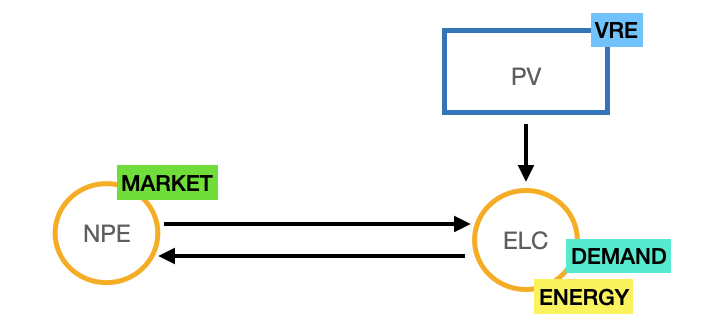
\includegraphics[width=0.8\textwidth]{Simple_house_company.png}
\caption{Graphical representation of the simple house company example set up.}
\label{fig:simple_house_company}
\end{figure}

In the example, we model two scenarios with four time steps. The first and second scenarios represent a sunny day and a cloudy day respectively. The solar energy availability capacity factor values for each scenario are seen in Table \ref{tbl:solar}. The demand time series is seen in Table \ref{tbl:demand}. In scenario one, the need for electricity is lower because due to the warmth of the sun the heating system is turned down. The market price estimates for the scenarios are seen in Table \ref{tbl:prices}. In the model, the scenario probabilities are 50\%.

The model optimises the usage of the photovoltaic system in both of the scenarios so that the costs faced by the house company. Notice that the VOM costs of the photovoltaic system in this example are 0 e/MW. Since this example is very simple, it is always optimal to generate as much energy as possible. This minimises the need to buy energy from the market and if there is excess energy, then that can be sold to the market.

\begin{table}[H]
\caption{CF time series representing solar energy availability.}
\label{tbl:solar}
\centering
\begin{tabular}{ l | l l l l }
Scenario    &   $t_1$ &   $t_2$ &   $t_3$ &   $t_4$\\
\midrule
1 & 1.0 & 0.90 & 0.90 & 1.0 \\
2 & 0.4 & 0.8 & 0.5 & 0.6 \\
\end{tabular}
\end{table}

\begin{table}[H]
\caption{Demand time series representing the house company's need for electricity.}
\label{tbl:demand}
\centering
\begin{tabular}{ l | l l l l }
Scenario    &   $t_1$ &   $t_2$ &   $t_3$ &   $t_4$\\
\midrule
1 & -19 & -19 & -18 & -17 \\
2 & -23 & -24 & -22 & -22 \\
\end{tabular}
\end{table}

\begin{table}[H]
\caption{Electricity market price estimates.}
\label{tbl:prices}
\centering
\begin{tabular}{ l | l l l l }
Scenario    &   $t_1$ &   $t_2$ &   $t_3$ &   $t_4$\\
\midrule
1 & 13 & 13 & 13 & 13 \\
2 & 13 & 13 & 14 & 12 \\
\end{tabular}
\end{table}


\subsection{Bidding constraint testing example}

The bidding constraint example is exactly the same as the simple house company example described above. In this case however, the model is run twice: once exactly as in the previous example and once with the bidding constraints under inspection. The bidding constraints are seen in Equations \eqref{eq:bidEq} and \eqref{eq:bidIneq}. The HouseCompanyEnergyModel.jl provided the ground work to test these constraints, which were then found to behave incorrectly.

\begin{align}
     & \quad v^{flow}_{i, n, s,t} - v^{flow}_{n, i, s,t} = v^{flow}_{i, n, s',t} - v^{flow}_{n, i ,s',t} \ , \nonumber \quad \quad \quad \quad \text{if } c^{energy}_{n,s,t} =c^{energy}_{n,s',t} \\[0.5cm]
    & \quad \forall n \in N^{markets}, i \in N: \{(i,n), (n,i)\} \in F,  s \in S, s'\in S, t \in T 
    \label{eq:bidEq}
\end{align}

\begin{align}
    & \quad v^{flow}_{i, n, s,t} - v^{flow}_{n, i, s,t} \leq v^{flow}_{i, n, s',t} - v^{flow}_{n, i ,s',t} \ , \nonumber \quad \quad \quad \quad \text{if } c^{energy}_{n,s,t} < c^{energy}_{n,s',t} \\[0.5cm]
    & \quad \forall n \in N^{markets}, i \in N: \{(i,n), (n,i)\} \in F,  s \in S, s'\in S, t \in T 
    \label{eq:bidIneq}
\end{align}


\section{Additional comments for future developers}

As said in the introduction, this package at the moment only lays the ground work for modeling interesting problems.

Some thoughts that I've had but could not make up my mind about.
\begin{itemize}
    \item Could the process flow Constraints \eqref{eq:maxLoad1}-\eqref{eq:maxLoad2} and ramping Constraints \eqref{eq:rampup1}-\eqref{eq:rampdown2} only be applied to the output flows of the processes? It seems unnecessarily complicated to declare these constraints for the input and output flows when the efficiency constraint \eqref{eq:efficiency} relates these flows to each other.
    
    \item Should the process flow Constraints \eqref{eq:maxLoad1} and \eqref{eq:maxLoad2} have the capacity factor upper bound written into them instead of declaring Constraint \eqref{eq:cf_UB} separately? Would it be motivated to be more concise in this way? Of course this would require still writing out the CF upper bound constraint Constraint \eqref{eq:cf_UB} out for VRE processes.
    
    \item Should transfer flows have a maximum capacity?
\end{itemize}

\end{document}
